\documentclass[12pt,a4paper]{article}
\usepackage[utf8]{inputenc}
\usepackage{amssymb, amsmath, multicol}
\usepackage{mathtext}
\usepackage[russian]{babel}
\usepackage{graphicx}
\usepackage[shortcuts,cyremdash]{extdash}
\usepackage{wrapfig}
\usepackage{floatflt}
\usepackage{lipsum}
\usepackage{concmath}
\usepackage{euler}
\usepackage{tikz}  
\usepackage{longtable}
\usetikzlibrary{graphs}

\oddsidemargin=-15.4mm
\textwidth=190mm
\headheight=-32.4mm     
\textheight=277mm
\tolerance=100
\parindent=0pt
\parskip=8pt
\pagestyle{empty}
\renewcommand{\tg}{\mathop{\mathrm{tg}}\nolimits}
\renewcommand{\ctg}{\mathop{\mathrm{ctg}}\nolimits}
\renewcommand{\arctan}{\mathop{\mathrm{arctg}}\nolimits}
\newcommand{\divisible}{\mathop{\raisebox{-2pt}{\vdots}}}

\graphicspath{{pictures/}}

\author{Радькин Кирилл, Б01-005}
\title{Лабораторная работа 2.2.1. Исследование взаимной диффузии газов.}

\begin{document}
	\maketitle
	
	\paragraph{Цель работы:}
		1) регистрация зависимости концентрации гелия в воздухе от времени с помощью датчиков теплопроводности при разных начальных давлениях смеси газов; 2) определение коэффициента диффузии по результатам измерений.
		
	\paragraph{В работе используются:}
		измерительная установка; форвакуумный насос; баллон с газом (гелий); манометр; источник питания; магазин сопротивлений; гальванометр; секундомер.
		
	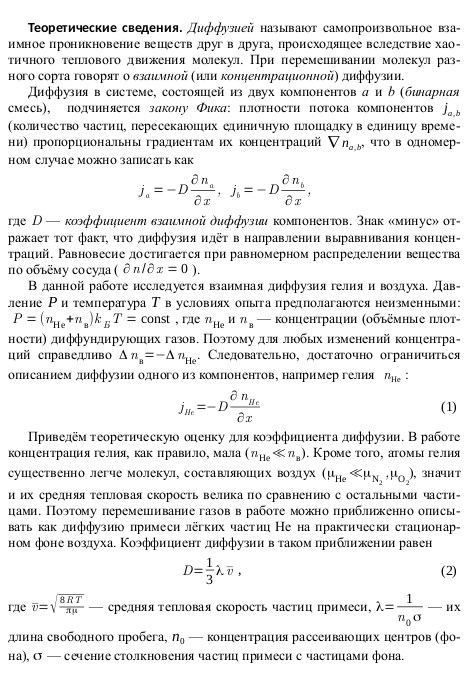
\includegraphics[scale=1.5]{1.png}
	\newpage
	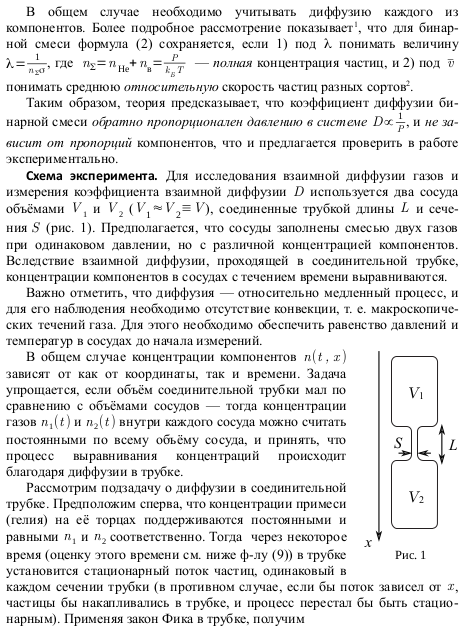
\includegraphics[scale=1.5]{2.png}
	\newpage	
	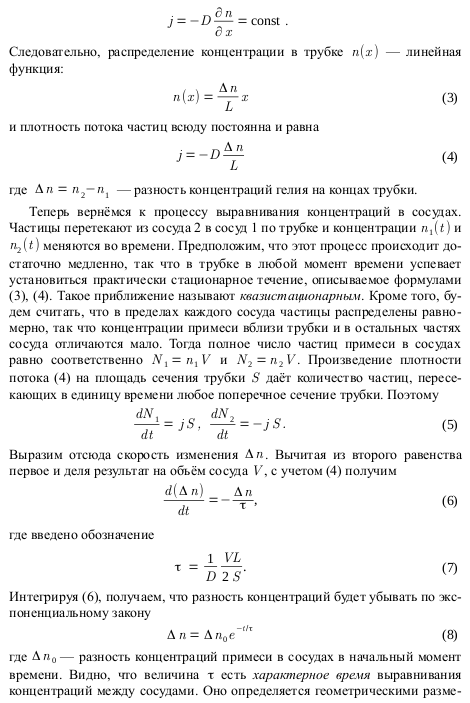
\includegraphics[scale=1.5]{3.png}
	\newpage	
	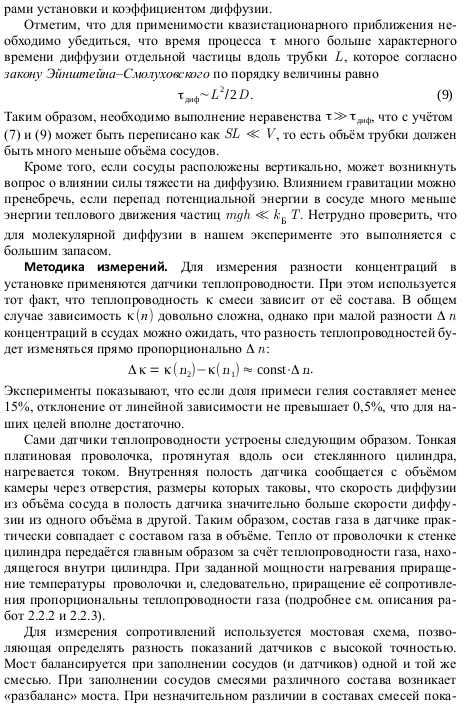
\includegraphics[scale=1.5]{4.png}
	\newpage	
	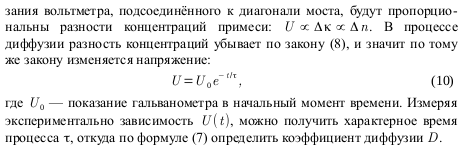
\includegraphics[scale=1.5]{5.png}
	
	\paragraph{Экспериментальная установка:} ~\\
	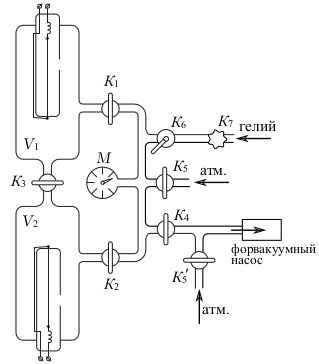
\includegraphics[scale=1.5]{Workplace.png}
	
	\paragraph{Ход работы:}
	\begin{enumerate}
		\item подготовим установку к работе.
		\item point Измерим показания вольтметра во время диффузии. Для этого будем настраивать вольтметр под рабочее давление $p_{\text{раб}}$, а после будем запускать в верхний сосуд водород с давлением $p_{H_2} = 0,2 p_{\text{раб}}$, в нижний --- воздух с $p_{\text{возд}} = 1,75 p_{\text{раб}}$, затем начинать процесс и ждать снижения показаний вольтметра на $30-50\%$. Повторим данные действия при нескольких рабочих давлениях: 1) 40 тор, 2) 100 тор, 3) 150 тор, 4) 200 тор, 5) 300 тор. Данные внесём в таблицу:
	
			\begin{longtable}{|c|c|c|c|c|c|} \hline
Время, c & 1 & 2 & 3 & 4 & 5 \\ \hline	
0 & 19.96 & 20.43 & 23.74 & 27.81 & 26.34 \\ 
10 & 19.35 & 20.13 & 23.45 & 27.65 & 26.13 \\ 
20 & 18.81 & 19.85 & 23.22 & 27.49 & 25.95 \\ 
30 & 18.27 & 19.56 & 22.99 & 27.36 & 25.73 \\ 
40 & 18.06 & 19.18 & 22.78 & 27.22 & 25.52 \\ 
50 & 17.25 & 19.01 & 22.55 & 27.07 & 25.32 \\ 
60 & 16.74 & 18.75 & 22.33 & 26.95 & 25.12 \\ 
70 & 16.29 & 18.49 & 22.13 & 26.81 & 24.92 \\ 
80 & 15.84 & 18.25 & 21.92 & 26.68 & 24.73 \\ 
90 & 15.41 & 18.01 & 21.73 & 26.55 & 24.59 \\ 
100 & 14.98 & 17.78 & 21.55 & 26.42 & 24.36 \\ 
110 & 14.56 & 17.54 & 21.37 & 26.31 & 24.18 \\ 
120 & 14.17 & 17.32 & 21.18 & 26.16 & 24.01 \\ 
130 & 13.79 & 17.11 & 21.01 & 26.04 & 23.83 \\ 
140 & 13.39 & 16.88 & 20.83 & 25.92 & 23.66 \\ 
150 & 13.03 & 16.68 & 20.67 & 25.79 & 23.49 \\ 
160 & 12.66 & 16.47 & 20.49 & 25.66 & 23.31 \\ 
170 & 12.34 & 16.25 & 20.32 & 25.54 & 23.14 \\ 
180 & 12.02 & 16.07 & 20.15 & 25.42 & 22.98 \\ 
190 &  & 15.88 & 19.98 & 25.31 & 22.83 \\ 
200 &  & 15.69 & 19.83 & 25.17 & 22.67 \\ 
210 &  & 15.49 & 19.66 & 25.05 & 22.51 \\ 
220 &  & 15.31 & 19.57 & 24.94 & 22.37 \\ 
230 &  & 15.12 & 19.34 & 24.82 & 22.21 \\ 
240 &  & 14.95 & 19.18 & 24.72 & 22.06 \\ 
250 &  & 14.76 & 19.02 & 24.61 & 21.91 \\ 
260 &  & 14.58 & 18.87 & 24.48 & 21.76 \\ 
270 &  & 14.41 & 18.73 & 24.37 & 21.62 \\ 
280 &  & 14.23 & 18.57 & 24.26 & 21.47 \\ 
290 &  & 14.06 & 18.42 & 24.16 & 21.33 \\ 
300 &  & 13.89 & 18.27 & 24.05 & 21.19 \\ 
310 &  & 13.73 & 18.13 & 23.94 & 21.04 \\ 
320 &  & 13.57 & 17.98 & 23.83 & 20.91 \\ 
330 &  & 13.41 & 17.83 & 23.73 & 20.76 \\ 
340 &  & 13.08 & 17.71 & 23.61 & 20.63 \\ 
350 &  & 12.93 & 17.43 & 23.51 & 20.49 \\ 
360 &  & 12.78 & 17.29 & 23.41 & 20.35 \\ 
370 &  & 12.63 & 17.15 & 23.31 & 20.22 \\ 
380 &  & 12.48 & 17.02 & 23.19 & 20.09 \\ 
390 &  & 12.33 & 16.88 & 23.08 & 19.95 \\ 
400 &  & 12.19 & 16.75 & 22.97 & 19.83 \\ 
410 &  & 12.06 & 16.62 & 22.87 & 19.71 \\ \hline
			\end{longtable}
	
		\item Построим графики $U(t)$ и $\log{U}(t)$. \\
			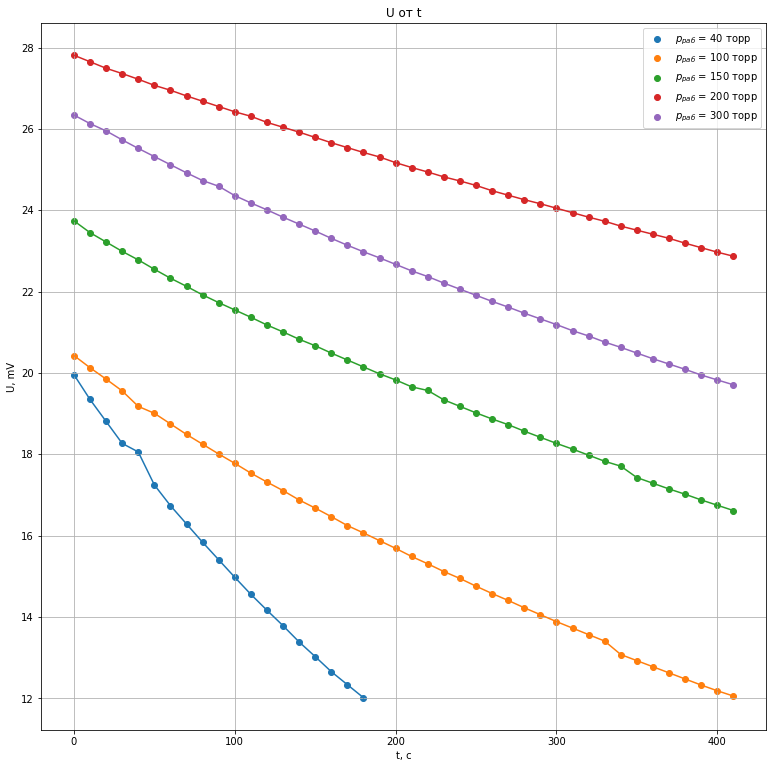
\includegraphics[scale=0.5]{ut.png} \\
			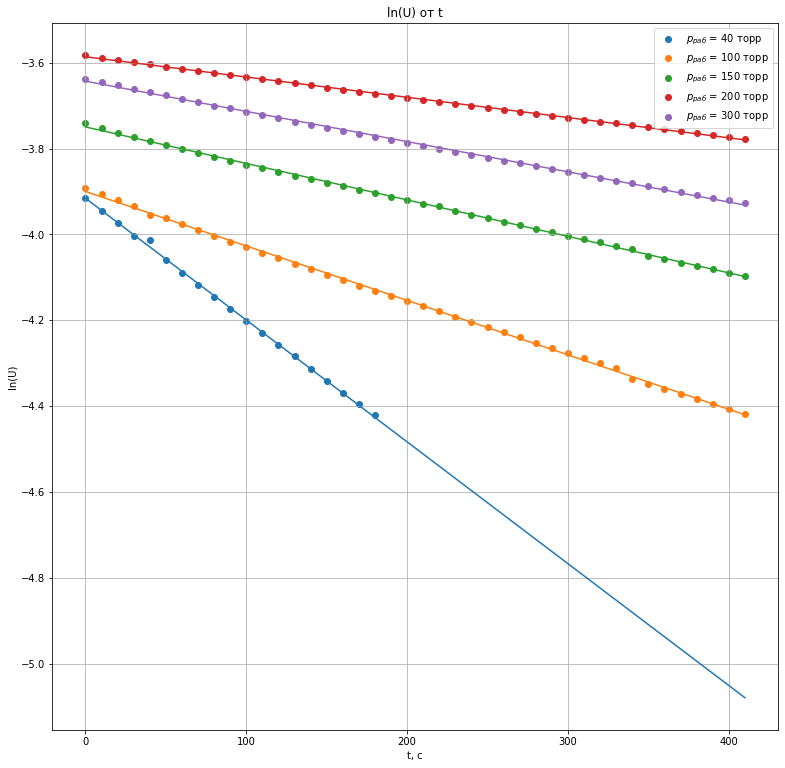
\includegraphics[scale=0.5]{lnut.png}
			
		\item Посчитаем коэффициенты взаимной диффузии по формуле $D = -\dfrac{kVL}{2S}$, используя параметры установки ($V = 1200 \pm 30 см^3, \dfrac{L}{S} = 5.5 \pm 0.5 см^{-1}$):
			\begin{itemize}
				\item $P_{раб} = 40$ торр: $D = 9.37 \pm 0.89$ $\dfrac{см^2}{c}$
				
				\item $P_{раб} = 100$ торр: $D = 4.18 \pm 0.39$ $\dfrac{см^2}{c}$
				
				\item $P_{раб} = 150$ торр: $D = 2.81 \pm 0.26$ $\dfrac{см^2}{c}$
				
				\item $P_{раб} = 200$ торр: $D = 1.56 \pm 0.15$ $\dfrac{см^2}{c}$
				
				\item $P_{раб} = 300$ торр: $D = 2.32 \pm 0.22$ $\dfrac{см^2}{c}$
			\end{itemize}
			
		\item Построим график $D\left(\dfrac{1}{t} \right)$:\\
			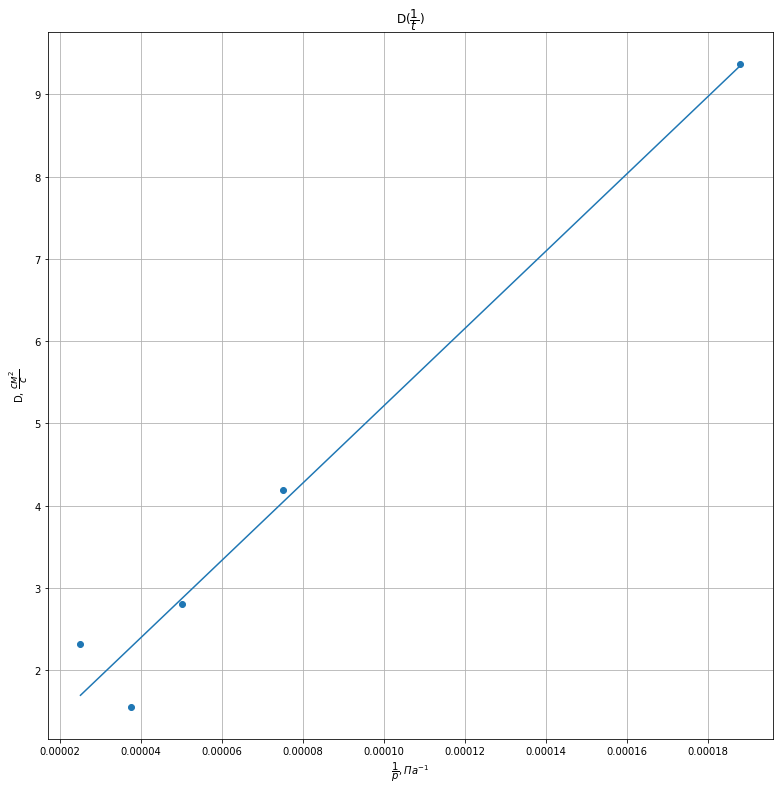
\includegraphics[scale=0.5]{dp.png}
			
		\item Посчитаем длину свободного пробега: \\
			\begin{equation*}
				\lambda = \dfrac{3D}{\overline{v}} = 3D \sqrt{\dfrac{\pi \mu}{8RT}} = 181 \pm 19 \text{ нм}
			\end{equation*}
			
		\item Посчитаем эффективное сечение столкновений $\sigma_{He-возд}$: \\
			\begin{equation*}
				\sigma_{He-возд} = \dfrac{1}{\lambda n} = \dfrac{kT}{\lambda P} = (2.2 \pm 0.2) \cdot 10^{-19} \text{ м}
			\end{equation*}
	\end{enumerate}
	
	\paragraph{Вывод:} ~\\
		При нормальном атмосферном давлении, наши вычисления дают нам значение коэффициента диффузии $D = 0.99$ $\dfrac{см^2}{c}$, что, в свою очередь отличается примерно на $50\%$ от табличного значения в $0.62$ $\dfrac{см^2}{c}$.
\end{document}